% !Mode:: "TeX:UTF-8"
\chapter{绪论}
我是绪论中的正文文本。

\section{课题背景}
我要使用引用命令为我的文章引用文献:
\ldots~加速度为~\SI{12345}{\square\micro\meter\per\nano\second},是一般加速度的\num{1.2345e3}倍~\supercite{Yablonovitch1987},误差~\SI{+-2e-6}{\square\micro\meter\per\nano\second}。

\subsection{该小节插图}
这里我要使用图形环境插图。注意该插图拥有中英双语图注和自动生成的图形编号。同时我要引用该图形:该图的编号是~\ref{fig-pcf}。
\begin{figure}[hptb]
 \centering
 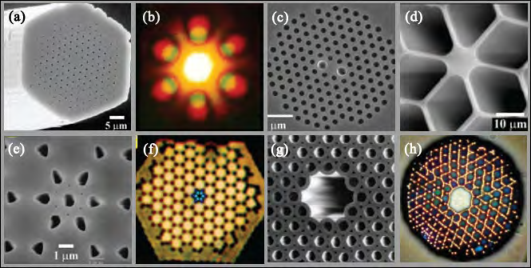
\includegraphics{chp-1_pcf}
 \caption{形式多样的光子晶体光纤。} \label{fig-pcf}
\end{figure}

\subsection{该小节插入公式}
我还要使用公式环境插入公式。注意公式是自动居中编号。同时我也要引用该公式,该公式的编号是~\eqref{equ-sample}
\begin{equation}\label{equ-sample}
\sum_{i=1}^n\sin\beta_i^2+\int_a^b\frac{D}{c}\,\mathrm{d}x=0
\end{equation}

\section{本章小结}
以上为本章的所有内容。